\section{Analytical Components of Agentic Visual Generation}
\label{sec:components}

The preceding section defined agentic visual generation as state-dependent control over a visual creation trajectory. This section examines the components through which that control is organized during visual creation. A typical trajectory contains a task requirement, a selected operation, an artifact or execution result, an inspection or check, and a subsequent decision, among other task-relevant events. The decision may keep the current plan, change an input or tool, repair part of the artifact, replan, stop, or take another permitted control action. One controller may perform these steps, or different components may handle planning, execution, inspection, and related functions.

For cross-paper comparison, we use six descriptive components. Goal Understanding, Specification, and Planning cover the task goal, constraints, dependencies, and planning records that guide later operations. Memory covers information and records retained for access at later decision points. Tool covers callable models, editors, code environments, applications, simulators, and related interfaces, together with their input conditions and returned execution information. Perception covers signal acquisition, observation, interpretation, diagnosis, verification, and acceptance evidence. Action covers artifact transformation, information acquisition, execution, environment interaction, communication, coordination, trajectory control, recovery, stopping, and related operations. Cross-Task Self-Improvement covers how information from a completed trajectory is carried into a later task: episodic reuse retrieves earlier attempts or repairs, while cross-task self-improvement requires evidence that the update changes later behavior. 

Each component corresponds to a part of the formal trajectory: Planning structures the goal $g$ into commitments that later decisions condition on; Memory holds, in addressable form, the part of the accessible state $z_t=(x_t,s_t,h_t)$ that must survive across steps; Tool supplies the interface set $\mathcal{I}_t$; Perception computes the observation map $\mathsf{O}$ and returns the evidence $o_t$ on which the closed-loop criterion rests; Action applies the selected $a_t=(i_t,c_t)$ through the kernel $\mathsf{U}$; and Cross-Task Self-Improvement updates $\pi_\theta$ or extends $\mathcal{I}_t$ across trajectories.

Figure~\ref{fig:ch3-components} shows the six components and their control dependencies, organized around the evolving visual artifact and the external task environment.

\begin{figure}[t]
  \centering
  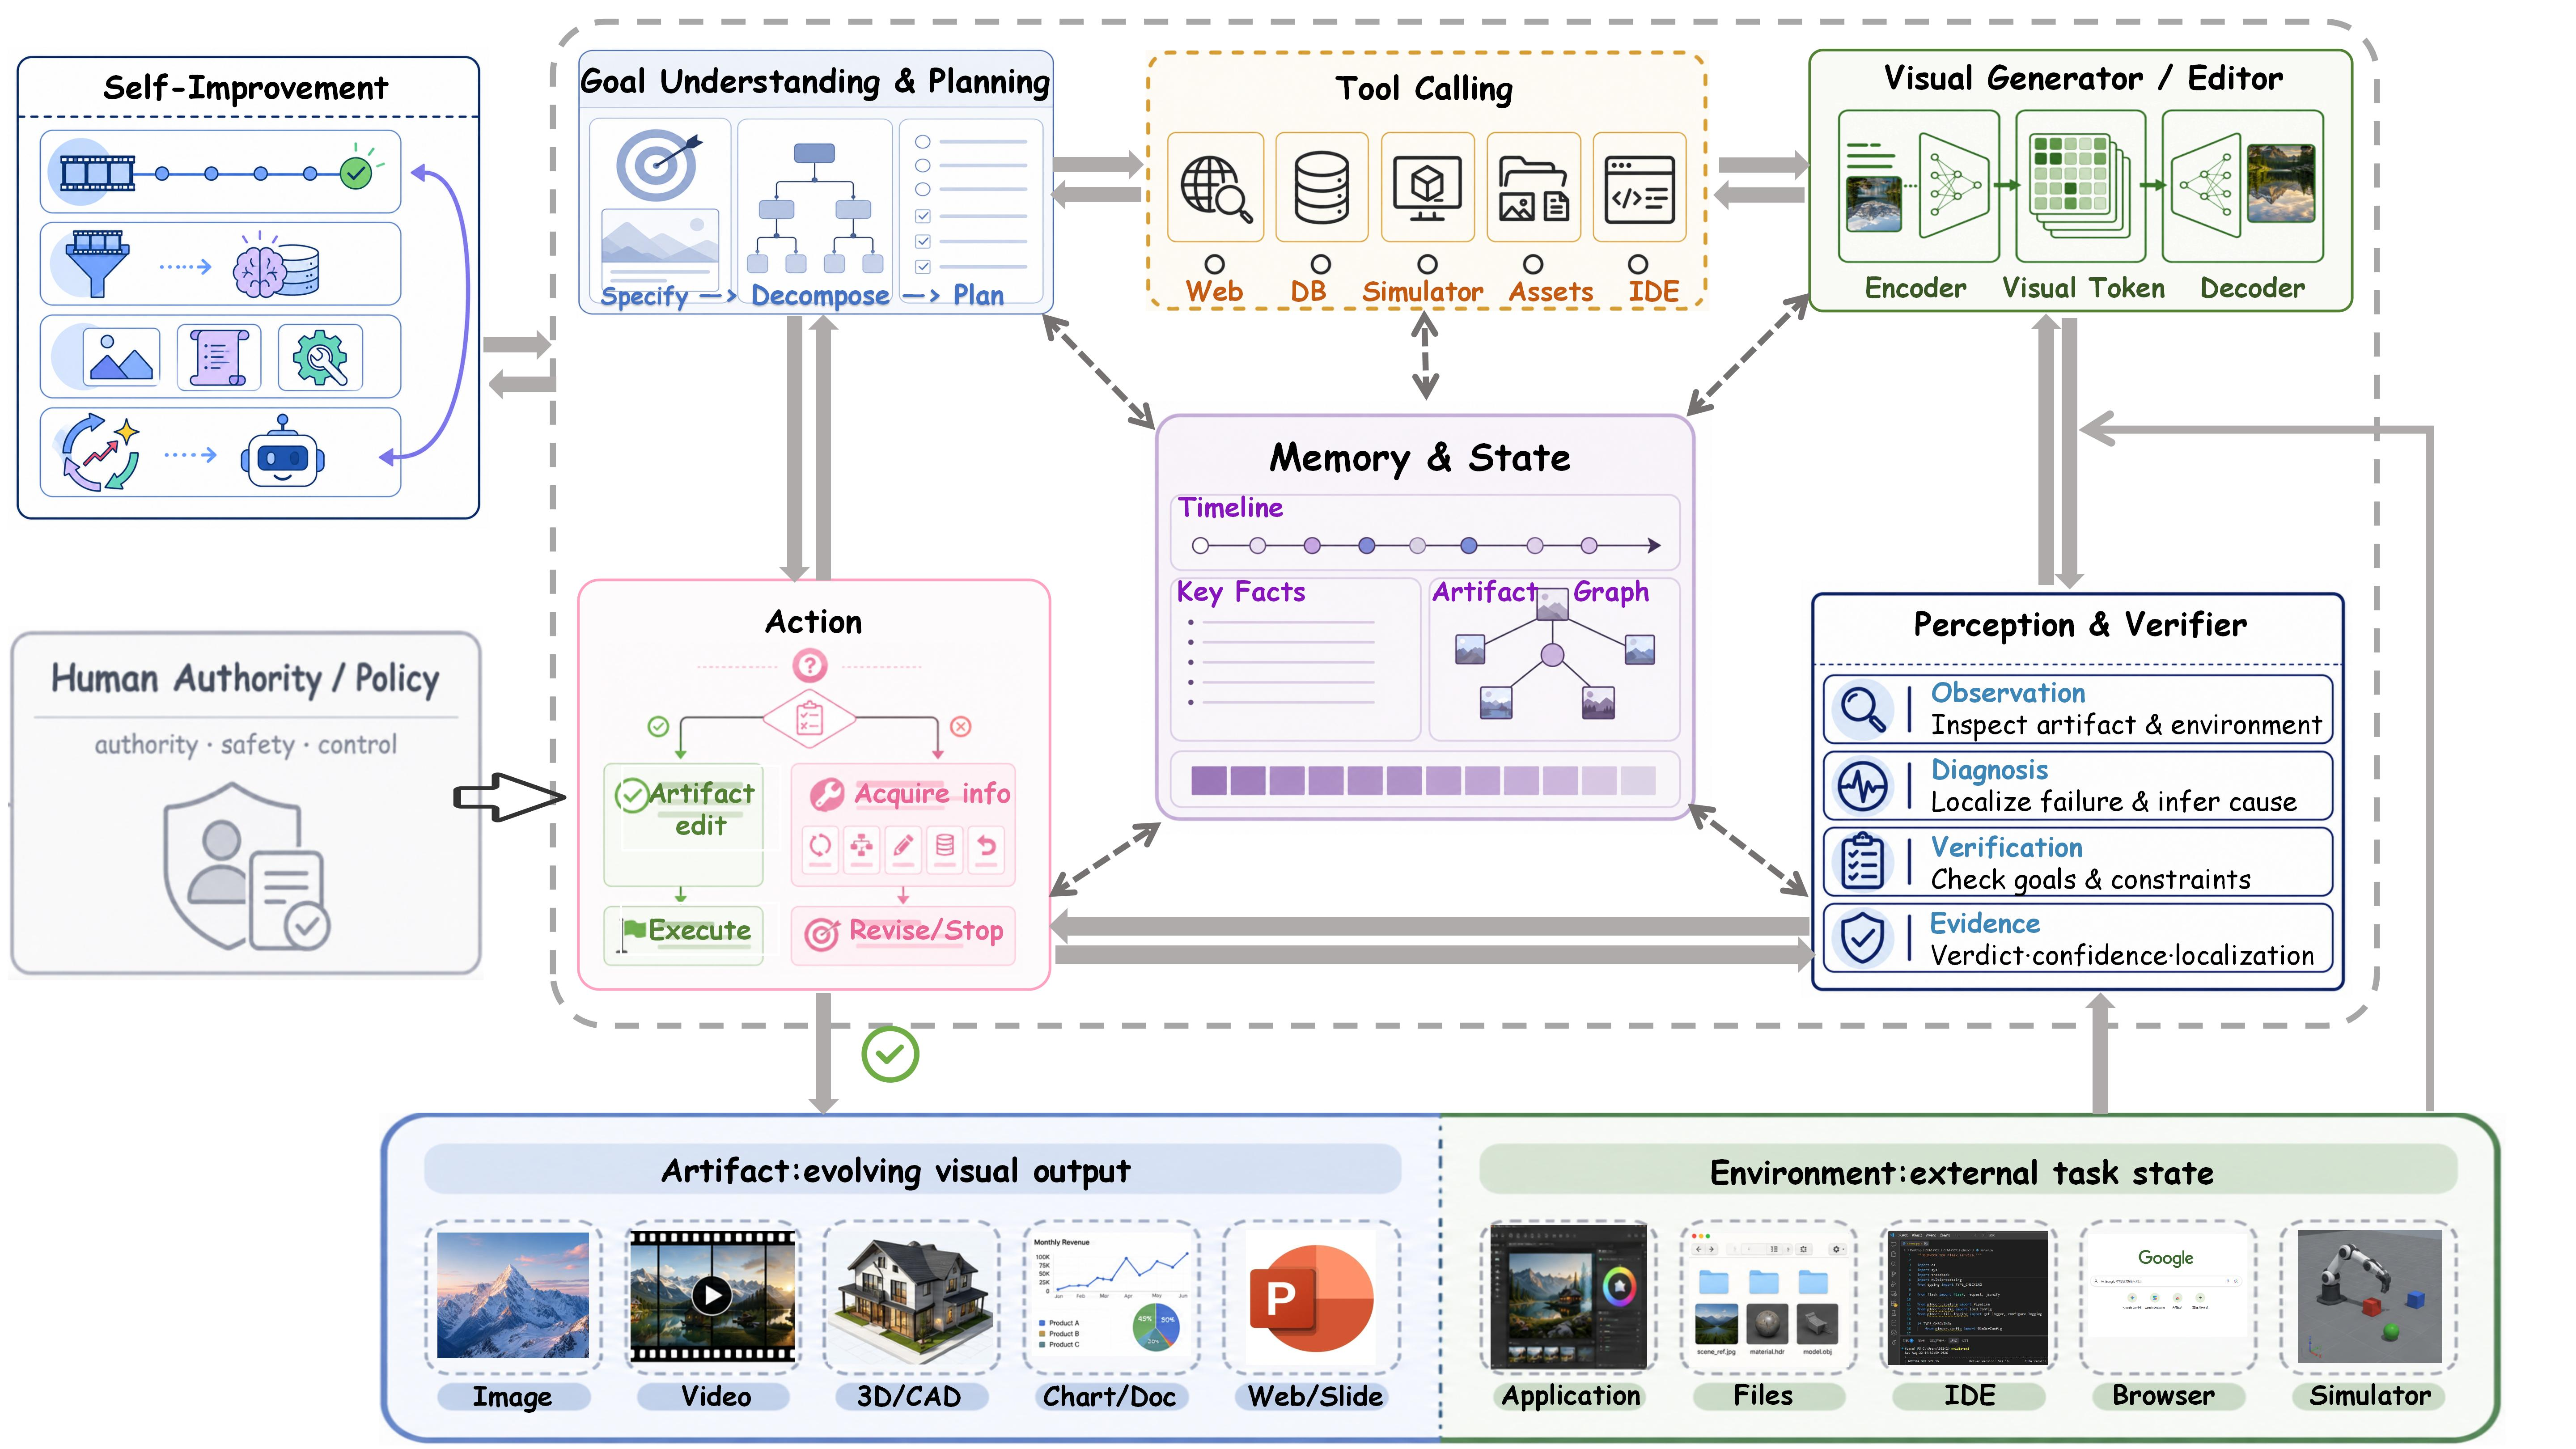
\includegraphics[width=\textwidth]{figures/ch3_components.jpg}
  \caption{The six components of agentic visual generation: goal
  understanding and planning, tool calling, memory and state, perception
  and verification, action, and cross-task self-improvement. The six
  components operate as a closed loop around the evolving visual artifact
  and the external task environment, with self-improvement carrying
  validated experience across tasks.}
  \label{fig:ch3-components}
\end{figure}


\subsection{Six-Component Analytical Framework}
\label{sec:analytical-framework}


\Needspace{7\baselineskip}

\subsubsection{Goal Understanding, Specification, and Planning}

\begin{keytakeaway}[Goal Understanding, Specification, and Planning]
This component transforms natural-language requests into provenance-marked commitments and a dependency-aware plan. By localizing repairs to specific failed commitments and keeping the plan revisable as new information arrives, it decouples the intended outcome from the distortions introduced by the generator's stochastic sampling.
\end{keytakeaway}


\textbf{Component definition.} This component interprets task information, expresses the intended visual outcome and its constraints, and organizes the remaining work into a plan. The input may combine a request, references, interaction context, domain requirements, and other task-relevant material at different levels of detail. The component turns this material into commitments that later operations can use, while keeping unresolved information attached to the part of the task it may affect. Its direct outputs include a current operational specification, unresolved items with their scope, and planned subgoals with their dependencies and order. When user information or task evidence changes a commitment or dependency, the affected specification and the remaining plan are updated along the same dependency structure.

A separate specification stage exists because natural-language requests compress intent through shared context: a sentence such as ``make the character look older'' fixes a target attribute while leaving composition, identity anchors, spatial relations, and rendering style to the generator's defaults, and those defaults are resolved silently during sampling. An explicit specification externalizes the defaults as commitments. Each commitment names the intended property, its priority relative to competing properties, and the acceptance condition under which a rendered artifact satisfies it. Planning compiles the commitments and their dependencies into subgoals; Perception supplies the verification evidence that checks these acceptance conditions at runtime, and Action applies the resulting evidence to the affected part of the plan. This externalization supports two downstream mechanisms. First, localization: a rendered artifact that deviates from intent maps to the violated commitment and, through it, to a likely cause, so the repair targets the cause with the intent re-derivation already done. Second, granularity: repair operates on whatever unit the specification names, so the specification determines the vocabulary in which a failure can be described. The weight of this stage in visual creation follows from the cost structure of the domain: a wrong commitment detected at sampling time costs a full forward pass through a stochastic generator, and because identity, style, and composition are entangled in the rendering process, a late-detected commitment failure also damages the properties that were already correct.

\textbf{Goal understanding.} Goal understanding converts an utterance into a task target by separating three provenance classes: what the user stated, what the system inferred from context and references, and what remains unresolved. This split is the provenance record on which later revision depends. Natural-language requests systematically rely on shared background: the speaker leaves composition, style, or scope unstated because they expect the listener to fill them in. A controller that treats the prompt as complete projects its own unstated background into the specification, and the projection hardens into a commitment whose origin is invisible. When a later revision must preserve user commitments while repairing system-inferred ones, an unmarked provenance makes the distinction unavailable, and repair can overwrite a user-stated constraint while attempting to fix a system-inferred one. Unresolved material is therefore surfaced at this stage and assigned a resolution route: a clarification request acquires the missing information; a scoped assumption records a provisional commitment together with the condition under which it holds; a deferred item stays attached to the commitments it affects, so clarification or new evidence can locate it later. Each route keeps the unresolved material addressable, which is what allows incoming information to be applied at the correct layer of the specification.

From Idea to CAD uses interactive requirements elicitation to clarify design intent from sketches and text before construction \cite{ocker2025ideatocad}. Search Beyond What Can Be Taught studies generator-specific knowledge gaps and trains a reasoner to decide when external search is useful; SearchGen-Bench evaluates search-augmented generation, while the co-training experiments study coordination between the search reasoner and the generator \cite{wang2026searchgen}. Clarify Before Executing detects incomplete or ambiguous 3D requests and asks targeted questions before tool orchestration, progressively turning the clarified intent into an executable workflow \cite{avg260716352}.

\textbf{Operational specification.} An operational specification turns the interpreted goal into verifiable commitments, and its design covers two mechanisms: the structure of its commitments and the repair granularity it makes reachable.

\paragraph{· Commitment structure.} Each commitment records the intended property, its priority relative to competing properties, the condition under which it holds, and its provenance. The priority field resolves conflicts locally: when identity preservation and a local edit compete for the same region, the priority determines the winner without renegotiating the rest of the specification. The provenance field keeps user-supplied and system-inferred material distinguishable, so a later revision can preserve one class while revising the other. Commitments form a dependency structure: a change to a high-level commitment propagates to the affected subgoals downstream of it, while a local change touches only the connected part of the plan. This structure is what keeps specification updates tractable across a long trajectory.

\paragraph{· Repair granularity.} The reachable repair granularity is set jointly by the unit that the specification names and the unit that the artifact representation can address. Repair needs an addressable target: the specification supplies the address (which commitment failed and where), and the representation supplies the storage (what structure exists to receive the change). An object-level specification over a layered representation supports object-level repair; a prompt-level specification over a pixel representation supports whole-output regeneration, because the representation exposes no element that a repair could address even when the specification names one. Specification granularity therefore has to be chosen with the representation in view, and when repair precision matters the two are designed together.

NEWTON identifies a specification bottleneck in physics-grounded video generation: the physical specification must provide sufficient, dynamically relevant, and verifiable information for the simulator and generator to realize the intended behavior \cite{feng2026newton}. Divide and Conquer makes the objects, attributes, relations, and scene layout of a compositional request explicit before composing the image \cite{wang2024divide}. MetaPoint converts a free-form image-editing request into structured object-level commands, including precise spatial information for the requested edit \cite{zhou2026metapoint}.

\textbf{Plan construction.} Planning compiles the specification into a dependency graph of subgoals, and its design covers three mechanisms: plan representation, decomposition depth, and the balance between alternatives and commitments.

\paragraph{· Dependency graph.} Each node carries the subgoal it addresses, its preconditions, the action intended to satisfy it, and the post-conditions that signal completion; edges record the order and the information dependencies among nodes. The plan may be written in natural language, as a program-like structure, as a tree, or as a hierarchy; the format matters less than the properties it exposes: order, dependency, and alternative continuation. These are what later decisions condition on.

\paragraph{· Decomposition depth.} Granularity is the central design variable, and hierarchical planning theory makes the trade-off precise: a plan is a decomposition in which compound tasks are refined into subtasks until primitive, executable ones remain, and the chosen depth determines how much work is decided before execution and how much is deferred to it. Visual generation sharpens this trade-off because intermediate artifacts are samples from a distribution. A plan that names a concrete intermediate appearance commits to one draw from that distribution and is invalidated when a different draw arrives; a plan that references dependencies, post-conditions, and acceptance conditions survives across draws, because those invariants hold regardless of which sample the generator returns. Robust visual plans therefore record alternative tools at each node and re-derivable lower-level decompositions, leaving leaf-level decisions to execution time. This is the contingent-planning pattern from partially observable domains, adapted to a setting where the observation step is a verification check performed by Perception on a rendered artifact.

\paragraph{· Alternatives and commitments.} Alternatives carry a cost that scales with their number: each recorded alternative enlarges the search space at execution time and the bookkeeping at plan time, while each additional commitment shrinks the space and forfeits adaptivity. The right operating point follows from the generator's variance and the cost of verification: a high-variance generator with cheap verification rewards alternatives; a low-variance generator with expensive verification rewards commitments.

GenArtist represents generation and editing operations in a planning tree, with sibling nodes encoding alternative tools for the same action \cite{wang2024genartist}; it operates at the alternatives-heavy end of the spectrum and pays with a larger search space. LightVA recursively decomposes an analytical request into data and visualization tasks for subsequent execution \cite{zhao2024lightva}. From Plans to Pixels generates structured atomic decompositions for open-ended, long-horizon image-editing requests and conditions tool and region selection on the resulting plan \cite{avg260515181}; it commits to one decomposition to make region-level tool selection tractable, giving up the alternative continuations that GenArtist preserves. Each occupies a defensible operating point given its generator variance and verification cost.

\textbf{Plan revision.} Planning remains revisable when new information changes a commitment, a dependency, or a condition governing the next action, and its design covers two mechanisms: the revision procedure and staleness detection.

\paragraph{· Revision procedure.} Revision theory distinguishes full replanning, which re-derives the plan from the current state, from plan repair, which applies a local transformation to the existing plan while preserving its valid parts. Repair is the cheaper option whenever the dependency structure can identify the subgoals downstream of the change; replanning is the fallback when the change invalidates the plan's top-level structure. The procedure follows the dependency graph: classify the incoming information as a refinement, a violation, or an addition to an existing commitment; locate the affected commitments; compute the affected subgoals (the downstream closure of the changed commitment); and re-derive only those subgoals, retaining the rest. The revision scope therefore equals the downstream closure of the changed commitment, which keeps the relationship between new information and the resulting planning decision explicit.

\paragraph{· Staleness detection.} A recurring failure is the stale plan. A plan is valid under the artifact state that held at construction time; execution mutates the artifact, so any subgoal whose preconditions referenced a mutated state becomes stale without an explicit invalidation event. The mechanism-level guard binds subgoal applicability to post-conditions evaluated at decision time: the precondition check itself detects staleness, and the damage stays local to the affected subgraph. When the incoming information is task evidence, such as a failed verification or an unexpected artifact, the revision is evidence-driven. When it is user information, the revision is preference-driven. Both follow the same procedure, and the distinction lies in who owns the resulting commitment.

Adaptive Task Reformulation changes the task representation and selects a new reformulation route when direct image editing fails \cite{avg260415917}. IMAGAgent orders constraint-dependent editing sub-tasks and uses reflection on intermediate results to trigger self-correction or retry \cite{avg260329602}. MIRA predicts one atomic editing action from the current visual state, feeds the updated image back into the next decision, and includes a stop decision when the instruction is satisfied \cite{avg251121087}.

Taken together, these four operations form a progression: task interpretation produces provenance-marked commitments, commitments compile into a dependency-aware plan, and incoming information updates the affected subgoals of the changed commitment. The resulting records provide the planning substrate that later operations condition on, while keeping unresolved assumptions and plan changes traceable to the information that produced them.


\subsubsection{Memory}

\begin{keytakeaway}[Memory]
Constrained by context budget, Memory manages the retention and injection of addressable information across the visual trajectory. Through the operations of formation, update, compression, deletion, and retrieval, it sustains task continuity and enables both episodic and procedural reuse for later decisions.
\end{keytakeaway}


\textbf{Memory definition.} Memory is information retained from an interaction so that a later decision can use it with the current task information. A record becomes memory when the system selects it from an interaction, gives it a readable and addressable representation, and makes it available at a later decision point. The retained information can describe a requirement, reference, visual observation, artifact version, action outcome, or prior experience. Its representation can be textual, visual, structured, executable, or multimodal, with links that preserve the relation between a record and the operation or result from which it came. Interaction history and current context provide source information; memory is the selected record that remains available for later use. In the formalization of Section~\ref{sec:agentic-visual-generation}, Memory realizes the parts of the accessible state $z_t=(x_t,s_t,h_t)$ that must survive across steps in an addressable form: it carries selected content from the write at one step to the read at the next, and because the observation map $\mathsf{O}$ reads from $h_t$ alongside $x_t$ and $s_t$, a retrieved record enters the next decision through the same channel as direct inspection of the artifact.

The design pressure that makes retention a selection problem is context budget. A visual trajectory produces frames, intermediate renders, tool traces, and verification outputs whose volume exceeds what a decision context can carry across turns. Retention is therefore governed by expected decision value: candidate records compete for storage and for injection cost at later decisions, and the records that survive are those whose expected contribution to a later decision justifies both costs.

Qwen-Image-Agent treats memory as a context-grounding source for historical and personalized information during image generation and editing \cite{avg260626907}. The Cognitive-structured Multimodal Agent externalizes visual information into episodic visual memory and uses a retrieval engine to reactivate relevant visual episodes across turns \cite{avg260708497}. LAVE maintains a memory buffer of prior conversations and combines recent history with the current instruction when constructing a video-editing action \cite{wang2024lave}. These systems show the same basic operation at different scopes: information produced earlier is selected and supplied to a later generation decision.

\textbf{Memory formation, update, compression, deletion, and retrieval.} Memory passes through five operations: formation, update, compression, deletion, and retrieval. These operations jointly determine what survives a trajectory and what reaches a later decision.

\paragraph{· Formation.} Memory formation selects information with potential future utility from a request, reference, action, artifact output, observation, feedback signal, or user correction. The selection may preserve an event, extract a proposition from it, summarize several related events, or link an editable source to the result it produced. The selection criterion covers the information's expected value for a later decision, together with its scope, reliability, and provenance. During a multi-turn image edit, the system retains a user-confirmed subject identity and a region that has already met the task constraints, and marks an unconfirmed stylistic preference as unresolved. During long-video creation, frame-level observations are collected as candidates and converted into a record about an entity or relation that persists across the relevant part of the trajectory.

\paragraph{· Update.} Updating incorporates new information into an existing record or set of records. It can append a new event, revise a value, attach evidence, change the validity interval, merge compatible entries, or preserve competing versions when the evidence is unresolved. Each update records the scope, source, and validity interval of the revised content, which makes staleness detectable at retrieval time, where the expired record is filtered before it reaches a decision. When a later edit changes the approved appearance of an object, the corresponding memory points to the new version while retaining the earlier version as provenance. When a new observation conflicts with an earlier one, the record holds both claims together with their scope conditions, and verification evidence from Perception closes the conflict at a later decision point.

\paragraph{· Compression.} Compression reduces the amount of stored information or the context supplied to a decision while preserving the content needed for that decision. Its operations include summarization, which replaces repeated observations with a stable description; deduplication, which merges records that express the same fact; and hierarchical storage, which links a compact summary to more detailed evidence. The two record classes divide the work: descriptive records are cheap to store and retrieve and support reasoning, while raw visual records carry appearance at higher storage and injection cost, and a description alone lacks the information needed to render the described content again. Hierarchical storage therefore links the description to its supporting frames, so reasoning steps retrieve the description and appearance-critical steps reach the frames through the link; a long sequence of consistent character observations is represented by a compact identity record with links to the frames that support it, and an exceptional frame remains available for diagnosis. The compressed record preserves the constraints, dependencies, uncertainty, and provenance required to recover or revise the relevant part of the artifact.

\paragraph{· Deletion.} Deletion removes a record, marks it inactive, or lets it expire when its validity, scope, utility, safety, or maintenance cost no longer supports retention. Local deletion removes an obsolete tool parameter or a failed intermediate version while the task requirement and the last verified artifact remain available. Conditional deletion retains a record for provenance while excluding it from ordinary retrieval after its validity interval ends, so the record stays available for audit and leaves the decision surface. Expiry based on the validity interval gives time-driven deletion without explicit removal.

\paragraph{· Retrieval.} Retrieval makes retained information available to a current decision. The query is constructed from the task specification, the current observation $o_t$, and the information needed for the next operation. Retrieval proceeds in stages: candidate records are matched on semantic distance, hard filters on scope, identity, and validity remove the records whose scope or validity interval fails the current decision, and post-retrieval processing orders, summarizes, and binds the remaining records to the current artifact. When a later shot is edited, retrieval returns the latest approved identity record, the relevant reference frame, and the prior repair that affected the same dependency, and unrelated experiments stay outside the decision context. Retrieval occurs at task initialization, at selected turns, or when a new observation creates a need for earlier evidence. Its role is complete when the returned record is available to the subsequent decision, such as choosing an input, editing a source representation, selecting a tool, revising a plan, or stopping. It does so as part of the observation $o_t$, on the same footing as evidence acquired directly from the artifact or the environment.

COMFYCLAW distills trajectories, execution errors, and verification feedback from image-workflow construction into reusable Agent Skills and progressively discloses those skills when later workflows require them \cite{avg260701709}. DataEvolver converts rejected text-rich image samples and their verification causes into semantic feedback, retains useful feedback entries, merges near-duplicate observations, and uses the resulting experience memory to revise later retrieval queries and generation prompts \cite{avg260631537}. VideoWeaver stores process and output evidence from long-video generation cases and uses the accumulated context to summarize category-level patterns and evolve reusable composition skills \cite{avg260608091}. These systems instantiate selected parts of formation, updating, compression, retention, and retrieval at different scopes.

\textbf{Memory types.} Memory types describe different properties of a retained record along three dimensions.

\paragraph{· Temporal dimension.} Short-term memory supports decisions within a turn or the current trajectory; long-term memory remains available across turns, scenes, or tasks. Both roles can be implemented by the same store when the formation and retrieval schedules attached to their records differ: a type is a property of the schedule attached to a record.

\paragraph{· Functional dimension.} Working memory holds the active task workspace; factual memory holds relatively stable information about users, environments, references, or visual entities; episodic memory holds particular attempts and outcomes; procedural or skill memory holds reusable action patterns. These four roles map onto the three functions described below: working and factual records carry task continuity, episodic records support episodic reuse, and procedural records support procedural reuse.

\paragraph{· Representation dimension.} Textual or token-level summaries preserve requirements and prior decisions; visual or multimodal records preserve appearance, identity, and visual evidence; structured records and graphs expose entities and dependencies; executable or artifact-linked records connect source code, workflows, or other editable representations to their outputs. The carrier decision follows from a property of visual content: identity is carried by appearance, a textual proxy preserves the decisions about a character, and the appearance that makes the character recognizable lives in the visual record, so the two classes are combined through links when both reasoning and appearance matter. Access can be private to one role or shared among several roles: private records carry role-local context, shared records implement the coordination surface among roles, and the shared partition carries per-record ownership and an update policy. The information channel can be textual, visual, structured, executable, or multimodal.

DreamFactory explicitly separates short-term information within a scene from long-term information that must persist across scene transitions, extracting a Base Description containing style, background, and character attributes and combining it with preceding-frame context for later key-frame generation \cite{xie2024dreamfactory}. ViMax uses global narrative context, retrieval-augmented generation, and graph-based cross-shot dependencies to carry story information into local video-generation decisions \cite{huang2026vimax}. ShareVerse implements spatiotemporal memory retrieval and conditions later video frames on retrieved memory frames to preserve a shared environment across asynchronous agent trajectories \cite{avg260302697}. Together, these examples cover temporal, functional, representational, and shared-access dimensions.

\textbf{Functions in agentic visual generation.} Memory in agentic visual generation serves three core functions.

\paragraph{· Task continuity.} Task continuity preserves requirements, references, identities, dependencies, artifact versions, and decision evidence that remain relevant as a visual creation trajectory proceeds. A later operation continues from an established task interpretation, inspects an earlier source or artifact version, preserves completed work, and revises the unresolved part of the trajectory. In a multi-turn image edit, a retained subject record and the latest verified image support a new local edit while the decisions established in earlier turns remain in force. In long-video creation, retained entity and scene records carry an established relation into a later segment while local content changes.

\paragraph{· Episodic reuse.} Episodic reuse retrieves a record of a particular earlier attempt, outcome, failure, or repair for a new but related request. The record supports the new request when its task conditions, selected actions, resulting artifact, and review evidence remain interpretable. A system retrieves a prior trajectory for a related visual defect, uses the successful intervention as an initial candidate, and adapts it to the current artifact and constraints; it also retrieves a failed episode to avoid repeating an action that produced the same conflict, or to select the observation that distinguished the earlier failure from a successful case. Consistent with the boundary fixed in the section introduction, the retrieval itself belongs to Memory, and the persistent adaptation that turns retrieved experience into a demonstrated later-task behavior change belongs to Cross-Task Self-Improvement.

\paragraph{· Procedural reuse.} Procedural reuse stores a reusable action pattern distilled from one or more episodes. The pattern can specify an operation order, preconditions, parameter relations, expected observations, or a repair strategy, while task-specific values are supplied by the current request. The form of retention determines what the pattern can do: retained as guidance, it informs how the next action is constructed; registered through tool creation as a callable capability with declared inputs and execution conditions, it enters the interface set $\mathcal{I}_t$ and extends the actions available to later decisions. A reusable visual-document skill, for example, preserves the sequence of inspecting source structure, rendering the result, checking the page, and revising the responsible source; a video-composition skill preserves continuity checks while the current scenes and assets change.

Agent Banana uses Context Folding to abstract a growing editing history into asset-, execution-, and planning-level records; its persistent ActionContext keeps the verified effective editing path and the associated image states for later turns, providing task continuity across successive edits \cite{ye2026agentbanana}. Generation Navigator represents each subsequent action using the original prompt, prior actions, generated images, reviewer feedback, and scores accumulated along the trajectory, keeping task-local evidence available for the next decision \cite{avg260517969}. SEAR builds a self-evolving episodic memory that consolidates high-reward restoration trajectories into retrievable expertise and uses a state fingerprint to select relevant prior trajectories, supporting episodic and procedural reuse across related restoration requests \cite{avg260628971}.


\subsubsection{Tool}

\begin{keytakeaway}[Tool]
Tools encapsulate visual-creation operations behind a boundary that defines input-output contracts and execution properties such as stochasticity and non-atomicity. By managing tool creation, selection, and routing, this component dictates the system's available capabilities and organizes execution across diverse artifacts, substrates, and coordination settings.
\end{keytakeaway}


\textbf{Tool definition.} This component represents a visual-creation operation as a callable tool and records the result of invoking it. The input to a tool call is constructed from the current task specification, the available task state, and the operation selected for the current subgoal. The tool boundary determines which inputs can be supplied, which artifact or environment is affected, and which outputs are returned to the ongoing trajectory. A returned result can contain a new or modified artifact, a structured state, an execution status, an error, or other information exposed by the executor. The interface may also expose preconditions, side effects, latency, cost, or reversibility, among other interface properties, when the implementation defines them. In the formalization of Section~\ref{sec:agentic-visual-generation}, Tool instantiates the interface set $\mathcal{I}_t$, and tool creation is the operation by which a new capability enters that set. A tool is a bounded, callable capability that carries out an operation on a visual artifact, an editable representation, or a task environment. Its design covers three mechanisms: the call and return contract, the addressability of results, and the execution properties that visual generators add to the contract.

\paragraph{· Call and return.} A tool's definition connects an operation name or endpoint to an input representation, an execution procedure, and a return representation. The input can be a prompt, image, mask, structured record, program, parameter set, or another task-specific value. The output can be a rendered result, an edited source, a geometric object, a chart, a document, an interface state, a simulator trace, an execution message, or another task-specific result. For example, an image-editing tool may accept a source image, a mask, and an edit instruction, invoke an editor, and return an edited image with the version or file identifier needed for the next call. A CAD tool may accept a parametric program and return geometry together with compiler or kernel status.

\paragraph{· Addressable results.} A useful interface keeps the relationship between the supplied input and the returned result addressable, so a later operation can identify the artifact version or environment state produced by the call. The interface can expose validation rules and failure states at the boundary, while the interpretation of whether a result satisfies the task remains a separate operation.

\paragraph{· Stochastic and non-atomic execution.} Visual generation adds two execution properties to this contract. First, the generation tools behind visual creation are stochastic. The same input to a diffusion-based generator can return different artifacts across calls, and even a fixed seed does not guarantee identical output across hardware, precision, or serving configurations. This has three direct consequences for the interface contract. A retry under the same condition draws a new artifact and does not recover the failed one. Verification is stated over the output distribution, and a single artifact is one sample against it. The interface returns the artifact itself, because the controller needs the concrete version to decide the next step. Second, tool calls can be non-atomic in real execution environments. A call may time out after the underlying operation has partially taken effect. This makes idempotency and version identification part of the interface contract. Repeating the call should have the same intended effect on the recorded state as a single call, and version identification binds each recorded state to the specific draw that produced it.

GenClaw provides an example of code-driven image operations in which a visual instruction is translated into executable operations over a canvas representation \cite{ye2026genclaw}. TOOLCAD formulates text-to-CAD interaction around tool calls to a CAD engine and uses trajectories containing tool execution outcomes \cite{gong2026toolcad}. CAD-Assistant connects a vision--language model to executable CAD functions so that language decisions produce CAD operations and returned model states \cite{mallis2024cadassistant}. These systems expose different interfaces, while each makes the operation boundary part of the available execution space. GenClaw and CAD-Assistant sit at two ends of the boundary spectrum. The former wraps pixel-level operations and carries their stochasticity at the interface. The latter wraps deterministic kernel calls, where reproducibility is available and geometric validation replaces distributional verification.

\textbf{Tool types.} Tool types describe the operation supplied by an interface and the substrate in which it executes. The classification covers two mechanisms: the function groups an interface can join, and the cost profile that the group separation produces.

\paragraph{· Function groups.} For agentic visual generation, the working groups include visual generation and editing tools; visual perception and analysis tools; retrieval and external-information tools; code, application, and rendering execution tools; and simulation or task-environment tools, among related tool functions. The groups describe the function provided to the current trajectory. One interface can combine several functions, such as an application tool that accepts editable code, renders a visual artifact, and returns execution messages. A perception or analysis tool contributes an output such as a measurement, label, relation, data summary, or another task-relevant signal. That output can inform a later decision when it is related to the current task requirements and available state.

\paragraph{· The five groups.} Visual generation and editing tools produce or modify the artifact used by the task; a call may map a prompt and reference image to a new image, or a source frame and edit region to a revised frame. Visual perception and analysis tools expose properties of an artifact or its source; examples include returning detected objects, text, measurements, or a data summary. Retrieval tools supply references, examples, or external information that can be used to construct later inputs. Code, application, rendering, and application tools execute programs or operate within an application environment; a plotting tool can turn a table and Python code into a figure, while a presentation tool can turn source code into rendered pages. Simulation tools execute a candidate representation under a modeled environment and return a trace or status that can be passed to a later decision; a physics tool can receive an event program and return simulated positions, contacts, or an execution failure.

AMACE uses separate agents for chart-code generation, chart rendering, and chart-quality assessment \cite{namgoong2025amace}. PlotGen combines code generation with numeric, textual, and visual feedback agents for scientific visualization \cite{goswami2025plotgen}. METAL separates chart generation, visual critique, code critique, and revision in a chart-to-code workflow \cite{li2025metal}. These examples show how tool type is determined by the operation and execution substrate, while the same system can expose several related interfaces.

\textbf{Tool creation.} Tool creation constructs a callable capability that can be registered and invoked by a later decision. Its design covers three mechanisms: the construction routes, the timing and scope of registration, and the composition of primitives.

\paragraph{· Construction routes.} The construction process may generate an implementation, wrap an existing model or application programming interface, compose several primitive operations, or attach an input--output interface to an executable procedure, among other constructions. It receives the intended operation, its dependencies, and the values that must cross the interface. It produces a callable object together with the information required to invoke it, such as accepted arguments, return format, environment requirements, and reported execution states, together with related interface metadata. Tests, example calls, or other checks can establish that the new interface is executable before it is placed in the available action space. A generated image, a source program, a workflow description, or a memory record can contribute to this process when the system uses it to implement, parameterize, document, or test a callable operation.

\paragraph{· Timing and scope.} Tool creation can occur before a task, when a system prepares a library of domain operations, or during a task, when an unavailable operation is assembled from accessible components. For example, a system can wrap a renderer as a callable function that accepts source code and asset paths, runs the renderer in a specified environment, and returns page images plus an execution status. A newly created tool can be specialized to the current artifact, generalized for later requests, or composed into a higher-level operation, among other scopes. Its utility depends on the compatibility between its input and output representations and the state of the execution environment. The record preserves the implementation version, dependencies, invocation conditions, and returned status needed to reproduce a later call. Tool creation supplies an additional callable capability; selecting when to use it and interpreting its result are separate decisions.

\paragraph{· Composition and localization.} Composition combines primitive operations behind one interface. A composed tool hides the internals of its primitives from the controller, which reduces interface complexity but also removes the localization information a later repair would need when the composed call fails midway. The composed interface must therefore record this provenance explicitly, noting which primitive produced which intermediate result and with what inputs, to preserve repairability when composition depth makes internals opaque.

\textbf{Tool selection and routing.} Selection identifies the capability for the current subgoal, and routing fixes the path the task travels through that capability. Both are established from the task and revisable as runtime evidence changes the requirements for the next operation.

\paragraph{· Selection.} Tool selection identifies the capability used for the current subgoal. The selected capability may be a generator, editor, analysis function, retrieval service, application, simulator, or another available executor. Selection uses the task requirements, current artifact and state, interface compatibility, and operating constraints such as quality, cost, latency, or side effects. Its output is a tool choice together with the arguments and conditions needed for invocation. Selection quality is bounded by two orthogonal limitations. An incomplete $\mathcal{I}_t$ leaves the correct capability unavailable regardless of the selection policy. An underspecified interface description leaves the correct capability present while its contract goes unrecognized. Tool creation addresses the first limitation, and interface documentation addresses the second. An interface description records the accepted input representation, the return representation, and the reported execution states in machine-processable form, which lets the selection policy match a subgoal to a capability from its declared contract.

\paragraph{· Routing.} Routing describes how the task or intermediate result is sent through the selected capability or a sequence of capabilities. A route can connect one tool directly to the next operation, pass an artifact through several compatible tools, or direct different subgoals to specialized paths. Selection therefore answers which capability is used. Routing describes the path, ordering, and handoff through which that capability participates in the task. Both can be established from the initial request and can be revised when an artifact, execution status, error, or other runtime information changes the requirements for the next operation.

\textbf{Tool use across artifact, execution, and coordination settings.} Tool use is organized along three dimensions: the artifact being produced or edited, the execution substrate, and the organization of tool calls.

\paragraph{· Handoff.} Tool use is the invocation of a selected capability and the handoff of its returned result to the next operation. The handoff preserves the representation needed by the recipient: an image or video render can be passed as a visual artifact, source code as an editable representation, a chart table as structured data, a CAD program as executable input, a simulator trace as an environment result, or another task-specific representation. The return record can include success or failure status, changed files or objects, generated artifacts, execution metadata, or related execution information exposed by the interface. A later operation can then continue from the returned state, supply a revised input, select another compatible tool, or deliver the artifact to the user.

\paragraph{· Artifact dimension.} The first dimension is the artifact being produced or edited. Pixel and temporal artifacts include images, masks, reference frames, clips, and scene segments. Structured artifacts include source code, layer hierarchies, scene descriptions, geometric programs, data mappings, layouts, and interface states. A portrait-editing call may combine a source image, a subject mask, and an edit instruction, then return a new image and an editable region for another local change. A CAD call may pass a parametric program and return geometry with compiler or kernel status. A chart, presentation, or Web call may pass data and source code and return a figure, rendered pages, or an updated interface state.

\paragraph{· Execution substrate.} The second dimension is the execution substrate. A selected tool can call a model or API, run code in a runtime or sandbox, operate a desktop or Web application, invoke a renderer, query an external information service, or execute a simulator or other task environment. A code-mediated operation can run a plotting script and return a figure plus execution status. An application-mediated operation can modify a slide or interface and return rendered pages or an updated state. A simulator-mediated operation can receive an event program and return a trace, contact states, or an execution failure. The handoff records the input representation, the executor, and the returned artifact or status so the next operation can address the correct file, object, or environment state.

\paragraph{· Call organization.} The third dimension is the organization of tool calls. One decision process can construct inputs and invoke tools directly. A staged workflow can pass the output of one operation to a later operation with a different interface. A multi-agent workflow can assign generation, editing, programming, rendering, or integration calls to different roles. Role decomposition purchases specialization at the price of the handoff. Each role boundary re-encodes the representation and ends the context the sending role treats as shared. The execution record therefore states what travels with the payload: the input, the acting role and tool, the returned artifact or status, and the decisions and constraints behind the artifact. Mora organizes model and agent roles for text-to-video, image-to-video, and editing workflows \cite{yuan2024mora}. GenMAC distributes compositional text-to-video work among collaborating agents \cite{huang2024genmac}. In such workflows, a prompt interpretation can be handed to a generation role, a generated result can be handed to an editing or integration role, and a rendered output can be handed to a later delivery step. The execution record retains the input, the acting role and tool, and the returned artifact or status so that each handoff remains traceable.

\paragraph{· Combined trajectories.} These dimensions can be combined in the same trajectory. A task may begin with a model call over a reference image, move to code execution for a structured layout, pass the result to an application renderer, and then use a simulator or interaction environment for a task-specific check. Across these combinations, the tool-use record identifies the operation invoked, the representation crossing the interface, the executor or role that acted, and the result made available for the next decision.

\subsubsection{Perception}

\begin{keytakeaway}[Perception]
Perception acquires and interprets signals from the artifact and execution environment to produce structured evidence. Through active signal selection, abductive diagnosis, and verification via exact and approximate oracles, it bridges the gap between observation and subsequent Action targets within the feedback loop.
\end{keytakeaway}


\textbf{Perception definition.} This component obtains and interprets information about a visual artifact, its editable representation, its execution process, the task environment, references, and interaction. Its input is a task-relevant signal source; its processing acquires, extracts, compares, localizes, or checks information; and its output is structured evidence that a later Action can use. This evidence may contain a score, a pass or graded status, a failed requirement, a location, a likely cause, uncertainty, supporting observation, or a candidate target. The mechanism can be instantiated for different visual artifacts and execution settings.

\textbf{Perception types and roles.} Perception types and roles covers the kinds of signals it operates on, and the role is fixed by its position in the perception-action loop: Perception supplies the comparator's evidence and Action applies the correction, so evidence production and correction execution are two stages of the same feedback loop.

Perception can operate on several kinds of information. Appearance perception concerns visible content, such as object presence, text rendering, color, texture, and layout. Structural perception concerns the representation that produced the visible result, such as source code, layers, scene relations, geometry, data mappings, or interface structure. Temporal and relational perception concerns changes across frames, shots, turns, entities, or dependent elements. Execution and environment perception concerns compiler messages, runtime status, application state, browser state, simulator traces, or other signals returned by an external process. Reference and user perception concerns comparisons with a supplied image, specification, example, preference, or correction. For example, in a slide workflow, the trajectory may combine page appearance, source structure, and parser status; a CAD workflow may combine rendered geometry, kernel measurements, and program state; a video workflow may combine sampled frames with identity and temporal relations. This type-based decomposition lets evidence be collected and combined per decision target, so that each check receives the signal class suited to its question and a coverage gap in one channel is covered by another.

\textbf{Signal acquisition and observation.} Signal acquisition and observation covers the selection of sensor channels and the trade-off among their coverage, timing, localization, and cost.

Signal acquisition obtains information from the artifact and its execution context. A system may, for instance, sample outputs at a fixed cadence, check a known risk point, select a crop or frame range, inspect source code or geometry, query a data record, retrieve a reference, or read a compiler, renderer, browser, application, or simulator result. The useful properties of a channel include its coverage, timing, localization, and cost. For instance, a scheduled render check may follow a scene transition, while a local inspection may be selected when uncertainty is concentrated in one region. These properties shape which signals are collected and when they become available for interpretation. The selection follows the active-perception principle: each acquisition carries a cost, and information gain depends on where the current uncertainty concentrates, so channel choice optimizes information value against acquisition cost. Scheduling cheap checks before expensive tests is the same optimization applied to the ordering of checks within a single verification pass.

In a program-mediated video workflow, Kubrick inspects Blender renders within its synthetic-video process \cite{he2024kubrick}. The artifact and execution substrate determine which signals become available for interpretation.

\textbf{Interpretation and diagnosis.} Interpretation and diagnosis covers the mapping from an acquired signal to a task requirement, a possible violation, and an affected part of the trajectory.

Interpretation connects an acquired signal to a task requirement, a possible violation, and an affected part of the trajectory. Diagnosis can identify a region, frame, object, component, or operation; associate the observation with a likely source; and retain competing hypotheses or confidence when the system reports them. The usefulness of a diagnosis depends on how directly it connects the observed signal to a later action target. Diagnosis proceeds by abductive reasoning: it generates the best-explanation hypothesis for the observed symptom, and when symptoms do not uniquely determine a hypothesis, the system retains competing hypotheses and selects the next check with the highest information gain. Root-cause localization accuracy directly determines the direction and speed of remediation: an incorrect judgment directs repair resources at an unrelated part, while an accurate one targets the violated commitment directly.

Concrete cases include CADSmith, which combines execution checks, CAD-kernel measurements, and visual assessment to separate runtime, dimensional, and morphological problems \cite{barkley2026cadsmith}; IterCAD, which uses executable sandbox feedback and geometric evidence in interactive CAD generation and editing \cite{hu2026itercad}; PhysAgent, which uses stage-specific simulation results to distinguish reconstruction failures from dynamics failures \cite{li2026physagent}; and DirectorBench, which organizes long-form video evaluation around checkpoint-level specifications and profile-aware bottleneck reports \cite{avg260530090}. These cases treat diagnosis as an interpretation of available evidence; the repair, retry, or route change remains a subsequent Action.

\textbf{Verification and acceptance evidence.} Verification and acceptance evidence covers the checking of acceptance conditions and the production of the corresponding evidence.

Verification checks an explicit requirement, acceptance condition, or property of the current result. Relevant targets include perceptual and semantic correspondence; relational, spatial, and geometric validity; temporal continuity and identity consistency; data, factual, and numerical fidelity; executable behavior and structural validity; physical plausibility; and human acceptance when a human review is part of the reported system. For a text-rendering requirement, this may involve OCR; for a CAD constraint, a geometry or compiler check; for a physical event, a simulator; and for an open-ended visual property, a learned judge or human review. Different targets require different evidence, and each check exposes a particular uncertainty.

A verification process can combine exact tests, reference-based comparisons, learned judges, source-level checks, simulations, and human review. It can record coverage, granularity, latency, confidence, and disagreement, and can schedule cheap checks before expensive tests. These checks answer different questions about the current result and can be combined when the artifact exposes multiple representations. Verification faces the oracle problem: a test oracle is a predicate that decides whether a behavior is acceptable, and for properties with an explicit specification an exact check serves as that oracle. For open-ended visual properties such as aesthetics or style consistency, no ideal oracle exists, so a learned judge or human review supplies an approximate oracle whose confidence and disagreement are recorded for Action to weigh at decision time.



\subsubsection{Action}

\begin{keytakeaway}[Action]
Action translates evidence and goals into state-changing operations across artifacts, environments, and communication channels. By executing artifact transformations, information acquisitions, and trajectory-control decisions, it performs the tangible modifications that drive the visual creation process forward.
\end{keytakeaway}



\textbf{Action definition.} Action is an operation selected at a decision point that changes a visual artifact, editable representation, external environment, available information, interaction history, or control trajectory. It receives the current goal and specification, Memory records, artifact and environment state, available Tool interfaces, and Perception evidence. It constructs an input, invokes an operation, and incorporates the returned artifact, state, status, communication result, or control update into the running trajectory. An action record can therefore identify the selected operation, its input and target, its executor or role when reported, its returned result, and available cost, latency, reversibility, or side-effect information. The action space includes artifact transformation, information acquisition, execution, environment interaction, communication, coordination, and trajectory control, among related operations.

\paragraph{· Operating arrangements.} The same action principle applies across several operating arrangements. A single decision process may invoke a model or editor directly; a staged workflow may pass a source representation through generation, rendering, and inspection; and multiple roles may divide generation, editing, programming, integration, or delivery. For instance, a reference image can be passed to a generator, the generated representation to a code or application runtime, and the rendered result to a later operation.

\textbf{Artifact actions.} Artifact actions covers the creation or modification of a visual artifact or its editable representation, and the two mechanisms it engages are the input-to-artifact mapping and the granularity at which the operation preserves or destroys completed work.

Artifact actions create or modify a visual artifact or its editable representation. The mechanism maps a task-specific input to a changed artifact while preserving the representation needed for a later operation. It can modify pixels, frames, masks, source code, layers, geometric programs, data mappings, layouts, or executable interfaces. A prompt and reference image can produce an image; a source frame, region, and edit instruction can produce a revised frame; a parametric CAD program can produce geometry and execution status; and data with source code can produce a figure, transformed data, or rendered pages. The operation may be global or localized, and its granularity determines which completed properties remain available for later steps. A destructive operation overwrites the intermediate state and leaves the overwritten content unrecoverable, so a later repair that targets an overwritten region must regenerate it. A non-destructive operation keeps the prior state addressable through a parameter record or a versioned layer, so a later step can roll back to it. A local edit touches only the selected region and preserves the completed properties outside it, while a global regeneration redraws the whole artifact and risks the properties that were already correct.

T2I-Copilot combines structured prompt interpretation, model routing, segmentation, interactive canvas operations, and quality evaluation in a text-to-image workflow \cite{chen2025t2icopilot}. AutoStudio separates prompt extraction, subject management, layout construction, layout supervision, and drawing for multi-turn image generation \cite{cheng2024autostudio}. Anywhere assigns distinct operations to foreground understanding, diversity enhancement, object-integrity protection, and text consistency in foreground-conditioned image generation \cite{xie2024anywhere}. The examples differ in artifact and operation, while each makes an artifact change available to later steps.

\textbf{Information acquisition actions.} Information acquisition actions covers the obtaining of material for a later operation, and the mechanism is the construction, dispatch, and return of a query or inspection request.

Information acquisition actions obtain material for a later operation. The mechanism constructs a query or inspection request, sends it to a source, and returns a reference, measurement, source fragment, preview, execution message, or other task-relevant record. It includes search and retrieval of references or external knowledge, data queries, source-code and file inspection, browser or application inspection, environment-state inspection, rendering of crops or previews, selection of a frame range, invocation of a perception or analysis service, and read or write operations on retained task records. For instance, a system may retrieve a visual reference before generation, inspect a source file before editing, or render a local crop before selecting a region-level action. Perception interprets the returned material; Action performs the operation that obtains it.

\textbf{Execution and environment actions.} Execution and environment actions covers the execution of an operation through a tool boundary, and the mechanism is the translation of a selected operation into an executable call that produces a state change.

Execution and environment actions operate through a model or API, a code runtime or sandbox, an application or browser, a renderer or compiler, a simulator, or another task environment. The mechanism translates a selected operation into an executable call, applies it to a target artifact or environment, and returns the resulting artifact, state, status, error, or trace. A CAD action can submit a program to an executable engine, an application action can modify a source file and render a page, and a simulator action can execute an event program and return a trace or failure. The Tool section defines the callable boundary; Action concerns the operation performed through that boundary and the state change it produces. When the operation produces side effects that are difficult to reverse, the execution environment can preserve a snapshot or checkpoint of the pre-action state, so a failed or undesired action can be rolled back to that state and retried with a revised input.

\textbf{Communication and coordination actions.} Communication and coordination actions covers the movement of information between roles or authority boundaries, and the mechanism is the selective forwarding of a payload across the boundary.

Communication and coordination actions move information between roles or authority boundaries. A sending operation selects what information to transmit, formats it for the recipient, and records the response or resulting handoff. The action can involve delegation, message passing, synchronization, aggregation, role handoff, delivery of an artifact or structured state, clarification requests, approval requests, rejection handling, progress reporting, or human override. In a multi-agent workflow, a prompt interpretation can be sent to a generation role, a generated result can be sent to an editing or integration role, and a rendered output can be sent to a later delivery step. Mora organizes model and agent roles for text-to-video, image-to-video, and editing workflows; GenMAC distributes compositional text-to-video work among collaborating agents \cite{yuan2024mora,huang2024genmac}. Because the channel between roles has limited bandwidth, the sending operation compresses or selects the payload, and the selection determines what the recipient can condition on; the evidence dropped at the boundary leaves no trace in the recipient's context, so the recipient cannot distinguish a silent exclusion from an absent signal.

\textbf{Evidence-conditioned action and trajectory control.} Evidence-conditioned action and trajectory control covers the use of Perception output to determine how the trajectory continues, and the mechanism is the mapping of evidence to an admissible response that drives the next state.

Evidence-conditioned action uses Perception output to determine how the trajectory continues. The mechanism receives a score, failed requirement, location, likely cause, or uncertainty, maps it to an admissible response, and performs that response. A critique can be sent to a prompt or code generator, a failed requirement can be applied to a local edit or revised input, an execution error can be passed to a retry or routing decision, and a result can be communicated to another role or user. A verified state can support continuation; an unresolved state can lead to more evidence, clarification, recovery, or stopping. The mechanism instantiates the belief-action coupling: Perception updates the agent's belief about the current state, and the policy selects the action with the highest expected value under that belief, so the verification verdict and its confidence enter the action choice through the same channel as the task specification.

\paragraph{· Trajectory-control actions.} Trajectory-control actions include tool, model, or role selection and routing; prompt, input, plan, dependency, or parameter updates; retry, branching, continuation, or path substitution; local repair, replanning, rollback, and bounded relaxation; stopping, termination, or deferral; and human authorization, override, or escalation. CoSTA* formulates multi-turn image editing as cost-sensitive tool-path selection \cite{gupta2025costa}. FaSTA* separates fast and slow tool paths and mines reusable subroutines for later editing decisions \cite{gupta2025fasta}. These systems treat trajectory control as cost-sensitive search over the action space, where each candidate action carries an expected cost and an expected reduction in remaining uncertainty, and the selected path balances the two.




\subsubsection{Cross-Task Self-Improvement}

\begin{keytakeaway}[Cross-Task Self-Improvement]
Cross-Task Self-Improvement converts completed trajectories into persistent behavioral changes for subsequent tasks. By forming reusable experience, attributing outcomes to specific decisions, and updating parameters or scaffolding components, it enables the system to adapt and generalize across diverse visual creation environments.
\end{keytakeaway}


\textbf{Cross-Task Self-Improvement definition.} Cross-Task Self-Improvement is a persistent change in a system's later-task decision process that is produced from experience collected in completed trajectories. Persistence means that the retained information, learned procedure, routing behavior, verifier behavior, or model state survives the completed trajectory and remains available when a subsequent task begins. The later decision can concern reference retrieval, prompt construction, tool selection, action ordering, verification, repair, or another task operation. Action covers corrections performed during the active trajectory. Memory covers information retained for later access. Cross-Task Self-Improvement covers the update that makes retained experience alter a later task decision. Within-action correction operates inside one selected operation. Within-trajectory iteration uses observations and feedback before the current request ends. Episodic cross-task reuse retrieves a prior case or trajectory for a subsequent request. Persistent system adaptation changes a reusable skill, routing rule, construction policy, verifier, or model behavior across subsequent requests. Final artifact quality is an outcome measure. Candidate selection is a decision inside the active trajectory. A later-task behavior change is the defining unit of cross-task self-improvement. The boundary separates two improvement branches: foundation-model improvement updates the model itself through parameter changes, and scaffolding improvement updates the surrounding components such as prompts, memory, tools, and executable agent logic, so the locus of change determines whether the update carries the cost of retraining or the cost of retrieval. The recent survey of self-evolving AI agents organizes this landscape along three dimensions, model-centric evolution (inference-based and training-based), environment-centric evolution (static knowledge, dynamic experience, modular architecture, and agentic topology), and model-environment co-evolution, which align with the two branches above and place visual-generation self-improvement within a broader taxonomy \cite{fang2025selfevolving}.

\textbf{Experience formation and attribution.} Experience formation and attribution covers the conversion of a completed trajectory into reusable information and the linking of observed outcomes to the actions that preceded them.

Experience formation converts a completed trajectory into information that can guide later decisions. The process records the task specification, references, intermediate artifacts, editable representations, tool calls, execution status, observations, diagnoses, verification results, critiques, repairs, costs, and user or evaluator judgments, together with provenance and task context. The formation process selects records with future decision value and compresses them into a case, a failure explanation, a repair relation, a preference, or another usable learning signal. Attribution links the observed outcome to the actions, conditions, and evidence that preceded it. This link attributes the observed improvement or failure to earlier choices, tool paths, repairs, and their conditions, and identifies the part of that relation that can be reused on a later task. The mechanism can compare successful and unsuccessful trajectories, align intermediate evidence with later outcomes, and discard records whose quality or provenance is unresolved. Attribution instantiates the credit assignment problem: it determines how the success or failure of an overall trajectory is distributed among the many earlier decisions that produced it, and because agentic trajectories span tens to hundreds of turns, episode-level attribution becomes uninformative and step-level signal must be recovered from outcome-level feedback. Agent-R addresses this recovery by using Monte Carlo tree search to splice a failed trajectory at its first error step with an adjacent correct path that shares the same parent node, so the model learns to reflect at the pivotal point where the deviation occurred rather than from the episode-level reward alone \cite{yuan2025agentr}.

GenEvolve compares multiple tool-orchestrated image-generation trajectories for the same request and extracts best--worst differences into structured visual experience covering search, reference selection, prompt--reference construction, and failure avoidance; the experience is supplied to a teacher branch that distills guidance into a student policy \cite{chen2026genevolve}. SIDiffAgent records complete diffusion-agent trajectories, summarizes pitfalls and successes at decision nodes, retrieves similar records, and injects corrective and workflow guidance into later prompts; its second episode uses the accumulated database on later benchmark prompts \cite{avg260202051}. These systems show experience formation as a sequence of logging, outcome attribution, abstraction, and later guidance construction.

\textbf{Reusable representations.} Reusable representations covers the forms in which retained experience is stored and the operational role each form makes available to a later task.

Reusable experience has several representation forms with different operational roles. A case preserves an episode, an artifact, a repair, or a tool trace for retrieval or replay on a related request. A strategy compresses recurring relations into a rule about search, reference choice, prompt construction, verification, or repair order. A skill packages a callable procedure, code fragment, workflow, or interface with inputs and execution conditions. The representation controls the amount of context carried into a later task and the degree of direct execution available to the system. Case reuse retains task-specific detail. Strategy reuse retains an abstraction that can guide several related tasks. Skill reuse exposes an executable operation that can be invoked as part of a later workflow. These forms instantiate the retention stage of the retrieve-reuse-revise-retain cycle: a solved problem is stored as a case or a compressed rule, the case enters a case base, and the case base makes the retained solution retrievable for a later similar problem, so the cycle closes only when retention has made the experience addressable for retrieval.

A long-video composition procedure can specify how clips, references, timing, and continuity checks are assembled. An image-editing correction rule can map a recurring defect to an edit operation and its parameters. A data-construction feedback rule can convert repeated rejection causes into the retrieval and synthesis choices for the next construction round. VideoWeaver refines and merges composition and creator skills from execution-trace and final-video evaluation, then tests the evolved skills on held-out task categories \cite{avg260608091}. COMFYCLAW distills trajectories, execution errors, and verifier feedback into a progressively disclosed skill library for ComfyUI workflow construction and validates the library on held-out prompts \cite{avg260701709}. The two systems instantiate skill-level reuse with different visual products and workflow interfaces.

\textbf{Retention, retrieval, and adaptation locus.} Retention, retrieval, and adaptation locus covers what survives a trajectory, how a later task queries it, and what changes after retrieval or learning.

Retention representation, access mechanism, and adaptation locus describe different parts of the update process. Retention representation specifies what survives a trajectory, such as an episode, summary, rule, skill, workflow, feedback record, or parameter state. Retrieval specifies how a later task queries that information, using signals such as task similarity, degradation-aware state fingerprints, artifact properties, tool compatibility, or temporal scope. Adaptation locus specifies what changes after retrieval or learning: the prompt, tool route, plan, verification rule, construction policy, skill library, or model parameters. An episode can therefore be stored in memory, retrieved by a state fingerprint, and applied as a prompt-construction change. A skill can be stored in a library, invoked through an interface, and used to alter tool ordering. A routing record can be retrieved from prior tool outcomes and used to select a generator. The retention form determines the adaptation channel: a record retained as context enters the later prompt without changing the model, a record retained as a skill enters the interface set as a callable capability, and a record retained as parameters enters the model weights through an update that persists across tasks, so the locus of retention fixes whether the later decision is changed by retrieval, by invocation, or by weight update. SEAL provides the parameter-level endpoint of this spectrum: the model generates a self-edit, a generation that may restructure information, specify optimization hyperparameters, or invoke tools for data augmentation, and the self-edit is applied through supervised finetuning as a persistent weight update; the self-edit policy itself is trained by reinforcement learning with the updated model's downstream performance as the reward, so the adaptation loop is closed entirely within the model's own generation and update \cite{pari2025seal}. AgentGym supplies the cross-environment analogue: a trinity of diverse environments, a trajectory set for prior capability, and an AgentEvol method that evolves the agent beyond previously seen tasks and environments, which places the parameter-level locus under explicit transfer and generalization tests \cite{xi2024agentgym}.

OctoT2I updates a text-to-image router through repeated evaluation and learning, retaining tool-use knowledge that changes later routing and supports new-tool integration \cite{jiang2026octot2i}. EvoIR-Agent organizes restoration experience in a hierarchical pool and retrieves it at multiple levels to guide later diagnosis and tool ordering \cite{avg260522208}. SEAR indexes explored restoration trajectories with degradation-aware state fingerprints and reuses the resulting episodic memory to reduce later search cost \cite{avg260628971}. DataEvolver retains verifier scores and rejection causes, summarizes them as semantic feedback, and feeds the updated feedback memory into later retrieval and targeted synthesis; the resulting construction data transfers to a second evaluated generator \cite{avg260631537}. These cases place the update at different loci while preserving the same sequence of retention, access, and later decision change.

\textbf{Transfer and evaluation.} Transfer and evaluation covers whether a retained experience changes a later task and whether the change remains useful under new conditions.

Evaluation determines whether a retained experience changes a later task and whether the change remains useful under new conditions. In-task improvement measures the quality change across revisions of one request. Cross-task transfer measures later requests after experience construction. Generalization tests unseen prompts, task families, tool combinations, generators, executors, or related environments. Persistence tests whether the update remains available after the original trajectory and across later sessions or batches. Safety evaluation measures forgetting, harmful updates, evaluator overfitting, retrieval contamination, and regressions on previously verified capabilities.

A causal comparison holds fixed the factors outside the claimed adaptation mechanism and varies the retained experience or update. The trace records whether the later run retrieves a different reference, selects a different tool or order, constructs a different prompt, changes a verification threshold, chooses another repair, or takes another related decision. Artifact evaluation measures constraint satisfaction, semantic alignment, structural validity, visual quality, and domain-specific properties. Process evaluation records calls, latency, cost, retries, recovery steps, and stopping decisions. Held-out task families, unseen tool combinations, independent evaluators, and human judgments test transfer beyond the trajectories used to build the update. Ablations with matched generators and sampling budgets separate retrieval effects, extra sampling, generator strength, and persistent policy or skill changes. Four failure modes bound the evaluation. Parameter-level updates face catastrophic forgetting: a weight update that optimizes the new task pushes parameters away from the values that were optimal for earlier tasks, so the stability-plasticity dilemma requires a balance between retaining old knowledge and learning new concepts. Experience reuse is not monotonically beneficial: when prior experience conflicts with the new task's conditions, negative transfer reduces rather than improves later performance. Verifier-driven improvement faces reward hacking: the agent overoptimizes the verifier's proxy reward without satisfying the latent objective, so the proxy score rises while genuine quality stalls. When the evaluation set overlaps the experience-construction set, retrieval contamination inflates the score and masks whether the update generalizes or merely retrieves a stored answer. Self-Rewarding Language Models instantiate the verifier-driven loop and its risk: the model uses LLM-as-a-Judge prompting to assign its own rewards during iterative DPO training, and the reported result is that both instruction following and the reward-modeling ability improve together across iterations, which is the intended regime; the same design also exposes the reward-hacking surface, because the verifier and the policy are the same model and a degenerate self-edit can raise the proxy reward without raising genuine quality \cite{yuan2024selfrewarding}.

VISTA supplies a test-time boundary case in video generation. Its procedure builds a temporal plan, generates candidate videos, selects a candidate through pairwise comparison, collects visual, audio, and contextual critiques, and rewrites the prompt for later rounds; its evaluation compares successive rounds on single- and multi-scene tasks \cite{long2026vista}. The reported adaptation occurs inside the test-time process. Persistent cross-task evidence uses a later-task retention test, transfer split, forgetting check, provenance record, and reversible update procedure.
